% Big Data Processing with Spark

\documentclass{sig-alternate}

\usepackage{hyperref}

\begin{document}
%
% --- Author Metadata here ---
\conferenceinfo{WOODSTOCK}{'97 El Paso, Texas USA}
%\CopyrightYear{2007} % Allows default copyright year (20XX) to be over-ridden - IF NEED BE.
%\crdata{0-12345-67-8/90/01}  % Allows default copyright data (0-89791-88-6/97/05) to be over-ridden - IF NEED BE.
% --- End of Author Metadata ---

\title{Efficacy/Analysis of Cloud-based Data-centric Frameworks for HPC Data Analysis}
%% \title{Alternate {\ttlit ACM} SIG Proceedings Paper in LaTeX
%% Format\titlenote{(Produces the permission block, and
%% copyright information). For use with
%% SIG-ALTERNATE.CLS. Supported by ACM.}}
%% \subtitle{[Extended Abstract]
%%\titlenote{A full version of this paper is available as
%%\textit{Author's Guide to Preparing ACM SIG Proceedings Using
%%\LaTeX$2_\epsilon$\ and BibTeX} at
%%\texttt{www.acm.org/eaddress.htm}}}

\numberofauthors{3} %  in this sample file, there are a *total*
% of EIGHT authors. SIX appear on the 'first-page' (for formatting
% reasons) and the remaining two appear in the \additionalauthors section.
%
\author{
% 1st. author
\alignauthor
Cameron~Christensen\\
       \affaddr{University of Utah}\\
       \affaddr{SCI}\\
       \affaddr{Salt Lake City, UT}\\
       \email{cchriste@sci.utah.edu}
% 2nd. author
\alignauthor
George~K.~Thiruvathukal\\
       \affaddr{Loyola University Chicago}\\
       \affaddr{820 N. Michigan Ave}\\
       \affaddr{Chicago, IL 60611}\\
       \email{gkt@cs.luc.edu}
% 3rd. author
\alignauthor
Venkatesh~Vishwanath\\
       \affaddr{Argonne National Laboratory}\\
       \affaddr{9700 S. Cass Ave\\
       \affaddr{Argonne, IL 60439}\\
       \email{venkat@mcs.anl.gov}}
}

\maketitle

\begin{abstract}

As dataset sizes grow, data analysis tasks in High Performance Computing
increasingly depend on sophisticated data-flows and out-of-core methods for
efficient system utilization. In addition, as HPC systems get larger, memory
access and data sharing are becoming performance bottlenecks. Cloud computing
is a data processing paradigm typically built on a loosely connected group of
low cost computing nodes without shared storage or memory. An emerging
exemplar in cloud computing is Apache Spark. In a sense, larger HPC systems
may start to look like very high performance clouds, and therefore we wish to
consider the potential of utilizing cloud frameworks in the context of HPC
data processing.

Our work proceeds by identifying common parallel analysis data flows for both
MPI-based and cloud-based applications, such as map and reduce. We construct
and perform several microbenchmarks to determine the performance
characteristic of these tasks using both types of system. In addition, we
compare the results for two real-world analysis tasks. The results of our
experiments are discussed in the context of their applicability to future HPC
architectures. Beyond understanding performance, our work is a demonstration that
technologies such as Apache Spark, while typically aimed at multi-tenant
cloud-based environments, can be used effectively in a traditional
clustering/supercomputing environment via the job scheduler. In the
case of Apache Spark, we also consider whether language plays a role,
especially when writing code in Python or Java/Scala.

\end{abstract}

% TODO: Get ACM categories right.
% A category with the (minimum) three required fields
\category{H.4}{Information Systems Applications}{Miscellaneous}
%A category including the fourth, optional field follows...
\category{D.2.8}{Software Engineering}{Metrics}[complexity measures, performance measures]

\terms{Theory}

\keywords{ACM proceedings, \LaTeX, text tagging}


% Everyting below here is from the Google doc. Still working on this (GKT).

\section{Overview}\label{overview}

Our goal is to understand and articulate the characteristics of
cloud-based dataflow processing in the context of HPC analysis tasks,
implement sample apps using spark, pegasus, and mpi and evaluate their
performance on both a supercomputing cluster and a cloud.

We will compare XYZ written in Apache Spark vs. MPI (a traditionally
used messaging middleware)

The microbenchmarks are chosen based on typical
computation/communication patterns found in HPC.

We're also looking at Python vs. Scala and whether there are any
performance differences.

Some words about tuning garbage collection. These folks seem to have
done some good legwork on same\footnote{https://databricks.com/blog/2015/05/28/tuning-java-garbage-collection-for-spark-applications.html}.

Also simply describe differences between implementation (e.g. lines of
code).

Out of core: Implicit in Spark

NOTE: we need to clarify what we mean by \emph{dataflow.}

\begin{itemize}
\item
  \begin{quote}
  Use in compilers:
  \href{https://en.wikipedia.org/wiki/Data-flow_analysis}{\emph{https://en.wikipedia.org/wiki/Data-flow\_analysis}}
  \end{quote}
\item
  \begin{quote}
  Dataflow architecture,
  https://en.wikipedia.org/wiki/Dataflow\_architecture
  \end{quote}
\end{itemize}

\section{Project Resources}\label{project-resources}

\textbf{Github:}
\href{http://github.com/cchriste/dataflow}{\emph{http://github.com/cchriste/dataflow}}

\textbf{Slack:}
\href{https://dataflowanalysis.slack.com}{\emph{https://dataflowanalysis.slack.com}}

\textbf{Google Docs:}
\href{https://drive.google.com/folderview?id=0BxLkEMNd9q6FfmpRaFZXSGlPc0JsSDdVdndCUm83SzN6UnlLVEk5T3ZsZmJ0VEVGREtNTkE\&usp=sharing}{\emph{dataflow\_analysis}}

\textbf{Dropbox:}
\href{https://www.dropbox.com/sh/odsd9uxe1elbhbf/AAD8J1TGuFY1VHJl2oPdm5E0a?dl=0}{\emph{spark\_hpc}}

My dropbox id is gkt@cs.luc.edu

\section{Dataflows}\label{dataflows}

\subsection{Components/Pipeline Stages}\label{componentspipeline-stages}

\begin{itemize}
\item
  \begin{quote}
  map
  \end{quote}
\item
  \begin{quote}
  flatmap
  \end{quote}
\item
  \begin{quote}
  reduce
  \end{quote}
\item
  \begin{quote}
  reducemap (ex: aggregation for file i/o)
  \end{quote}
\item
  \begin{quote}
  other?
  \end{quote}
\end{itemize}

\subsection{Multistage}\label{multistage}

Result of one computation feeds into the next, for example a \emph{map}
to another \emph{map}.

\subsection{Streaming}\label{streaming}

Computation performed over moving window.

\subsection{Evaluating Performance}\label{evaluating-performance}

Assessing the various components based on their rates of production and
consumption.

\subsection{To DAG or not to DAG}\label{to-dag-or-not-to-dag}

Some dataflows can have feedback..

\section{Dataflow Processing
Frameworks}\label{dataflow-processing-frameworks}

\subsection{Spark}\label{spark}

Spark is a general purpose cluster computing system similar to Hadoop.
It provides a new data abstraction that facilitates fast sharing and
history-based resilience, as well as an expanded set of data
transformation and actions, in addition to traditional map-reduce. In
addition, Spark provides a streaming processing abstraction as well as
bindings to common processing languages such as GraphX, R, and MLlib.

Spark is \emph{lazy,} and this philosophy underlies much of its design.
Computations will not be performed until their result is requested and
data will not be consolidated or repartitioned unless explicitly
requested.

\subsubsection{Running}\label{running}

Basics of job submission and execution.

\href{https://docs.google.com/document/d/1fq3z1-oEcCBhjKA__vl8LsVm3-uArJik7YFLYvYoN1Y/edit?usp=sharing}{\emph{running
spark on cooley}}

\href{https://docs.google.com/document/d/1lyzEHap1EznES0DKiMa3fsalepqPD6vnbZqSEMjCVPQ/edit?usp=sharing}{\emph{running
spark on magellan}}

\subsubsection{Resilient Distributed
Data}\label{resilient-distributed-data}

When a dataset is loaded by Spark, it becomes an immutable RDD. This
abstraction allows the data to be treated as a whole when in fact it may
be partitioned across many nodes of a distributed system. Each partition
also contains the history of transformations with which it was created,
called a \emph{lineage}, with which the partition can be recomputed if
necessary, such as in the case of a node failure. This lineage is a more
compact form of resiliency compared to data duplication as utilized by
Hadoop.

An RDD is split into \emph{partitions} whose size is at minimum the size
of a block on whatever storage device is being utilized (e.g. 32MB).
Each partition is further divided into \emph{records}, typically a
single line for text processing, or an entire binary file for binary
data. Binary data records can be explicitly specified. Large binary
files will be broken down into multiple partitions only if these
partitions can themselves be divided into records.

Spark distributes the blocks/data among the workers, if it does at all.

o is RDD different than Tachyon or do RDD blocks get written using
Tachyon (or HDFS, etc)?

o what data models does it support?

o how does it handle fault tolerance?

o what about transformation/views? (rows vs columns, more generally
chunks/blocks)

o when/how is the data replicated?

\subsubsection{}\label{section}

\paragraph{Storage Levels}\label{storage-levels}

RDDs can be stored in memory, on disk, a combination of the two, or off
heap (using Tachyon). MEMORY\_ONLY

Partitions that do not fit in memory will be recomputed from their
history when they are needed.

\paragraph{DISK\_ONLY}\label{diskux5fonly}

All partitions are stored on disk, just like Hadoop.

RDD partitions can be optionally replicated across up to two nodes. An
RDD partition must be small enough to fit

\paragraph{Persistence}\label{persistence}

RDDs can be persisted in memory for fast access between successive
operations. This is particularly important for iterative algorithms that
reuse some intermediate result. An RDD will be persisted according to
its specified storage level. Caches are cleared according to a least
recently used policy, or manually using RDD.unpersist()

\paragraph{Input}\label{input}

In order to get binary data into spark, we use the binaryFiles or
binaryRecords SparkContext functions. Both will read a directory filled
with binary files. The first will create one record per file, while the
second will partition files into records of an explicitly stated number
of bytes. For example, the following line will create an RDD with
partitions containing records of size float{[}3{]}:

vecs = sc.binaryRecords(sys.argv{[}1{]}, 12)

The binary data is read into a string. If you want to use the data as a
numpy array, the numpy.fromstring function can be used:

arr= np.fromstring(vec, dtype=np.float32)

This function can be used by RDD.map in order to convert the string
records into numpy records:

data = vecs.map(parseVector)

\subsubsection{Streaming}\label{streaming-1}

How to run spark in streaming mode.

\subsubsection{Spark and Tachyon}\label{spark-and-tachyon}

How do they work together? Are the performance characteristics
different?

Is it the same as ceph on Magellan? (ask Dan Olsen about ceph)

\subsection{Pegasus}\label{pegasus}

todo

\subsection{MPI}\label{mpi}

todo: reference implementation

\section{System Architectures}\label{system-architectures}

\subsection{Cooley}\label{cooley}

225Tflop cluster with 40Tb memory, shared disk + 355Tb local disk per
node, ...

\subsection{Magellan}\label{magellan}

7000 node cloud, no shared disk, per-node provisioning flexibility,
\ldots{}

\section{Sample Applications}\label{sample-applications}

\subsection{APS}\label{aps}

\begin{enumerate}
\def\labelenumi{\arabic{enumi}.}
\item
  \begin{quote}
  analyze image stacks from advanced photon source
  \end{quote}
\item
  \begin{quote}
  save results as IDX
  \end{quote}
\end{enumerate}

Our first sample application comes from a materials scientist who
utilizes the Advanced Photon Source (APS) to scan the construction of a
polymer material that could be used for nanoscale circuit printing. We
received an image stack from the APS as well as a sample Matlab script
and reproduced the results using the Spark framework.

Details can be found here.

\subsection{Bioinformatics}\label{bioinformatics}

\begin{enumerate}
\def\labelenumi{\arabic{enumi}.}
\item
  \begin{quote}
  look for patterns in genome streams
  \end{quote}
\item
  \begin{quote}
  and stuff
  \end{quote}
\end{enumerate}

\subsection{EVS}\label{evs}

\begin{enumerate}
\def\labelenumi{\arabic{enumi}.}
\item
  \begin{quote}
  look for patterns in genome streams
  \end{quote}
\item
  \begin{quote}
  and stuff
  \end{quote}
\end{enumerate}

\section{Evaluation}\label{evaluation}

\subsection{Pipeline Benchmarks}\label{pipeline-benchmarks}

\begin{itemize}
\item
  \begin{quote}
  map
  \end{quote}
\item
  \begin{quote}
  flatmap
  \end{quote}
\item
  \begin{quote}
  reduce
  \end{quote}
\item
  \begin{quote}
  reducemap (ex: aggregation for file i/o)
  \end{quote}
\item
  \begin{quote}
  other?
  \end{quote}
\end{itemize}

\subsection{Application Benchmarks}\label{application-benchmarks}

- data sizes

- data rates

- \# of stages

- system scale

- M:N coupling (in flatmaps/reducemaps, fan-in/fan-out degress)

- hw

- spilling?

- magellan vs cooley (shared storage vs node-level storage)

\section{Meeting Notes}\label{meeting-notes}

\emph{17Jun}

1.
\href{https://docs.google.com/document/d/1fq3z1-oEcCBhjKA__vl8LsVm3-uArJik7YFLYvYoN1Y/edit?usp=sharing}{\emph{spark
on cooley}}

- verify number of threads is actually correct, that we can
control/monitor threading

o identify multiple threads/worker

- try to load binary data (aps data or bio data)

o partition a huge binary file

o load a directory of smaller binary files

- use /projects/SDAV/cam directory, which is persistent

note: file(s) must be accessible to all workers, either through shared
path or hdfs/tachyon/etc

- when multiple files are read (or one big file is split) where does the
data go?

- dissect RDD (esp in context of binary blob):

o is RDD different than Tachyon or do RDD blocks get written using
Tachyon (or HDFS, etc)?

o what data models does it support?

o how does it handle fault tolerance?

o what about transformation/views? (rows vs columns, more generally
chunks/blocks)

o when/how is the data replicated?

- explore pipelines

1b.
\href{https://docs.google.com/document/d/1lyzEHap1EznES0DKiMa3fsalepqPD6vnbZqSEMjCVPQ/edit?usp=sharing}{\emph{spark
on magellan}}

- ceph (distributed file system looking thing, ask Dan Olsen about it)

- ...

2. spark streaming, pipelines

articulate pipeline stages (microbenchmarks):

- map

- flatmap

- reduce

- reducemap (e.g. aggregation for file i/o)

- ?

once we introduce, it makes sense to talk about rates of production and
consumption for each pipeline component, and how we can make them work
together sanely ("frame dropping", etc)

- add another stage, now rates of production/consumption matter

evaluate (application benchmarks):

- data sizes

- data rates

- \# of stages

- system scale

- M:N coupling (in flatmaps/reducemaps, fan-in/fan-out degress)

- hw

- spilling?

- magellan vs cooley (shared storage vs node-level storage)

3. plan for summer

- Try a real problem on both cooley and magellan, compare pros and cons.

- ideas: aps data analysis, biology data, and even convert it to idx at
the end and attach a visus viewer.

- could use an existing spark analysis (such as their machine learning
module), or create our own

Understanding the overall system and tradeoffs and how cloud-iness can
help hpc will be a good contribution.

- could also have an mpi app that does the same thing to compare
performance

week 3-7 - explore and code

week 8-9 - benchmarking (aps, bioinformatics, or both)

week 10 - write report/paper

w3:

- google doc

- pipelines/streaming investigation

- spark running on Magellan

- binary data importing and RDD dissection

w4:

- start APS/BIO

- pipelining/streaming benchmark

- explore pegasus a little. We know the project lead (Eva Delman) so we
can ask questions. This is mainly to have a notion of related work.

- rdd vs tachyon?

w5:

- refine aps/bio app

- identify analyses

w6:

- 2nd app (either the aps or the bio)

- (spillover from prev weeks)

w7:

- finish and have working apps

\emph{15Jun}

Pegasus mpi*, Legion, Uintah task graph,

Create a simulator using mpi/spark, try different dataflows

Different "feeds" produce at different rates,

Have different "coupling" characteristics (\#consumers vs producers)

Different primitives (join, scatter, etc)

Streaming (small chunks), dataflow (overall processing task)

Can we create a benchmark to characterize these types of *in-memory*
pipelines using these building blocks with their given characteristics?

Including not only dag but also feedback loops.

Challenge is to separate performance from effectiveness of pipeline.

We can try this using both spark and Pegasus using Cooley and Magellan.

Magellan has a lot of flexibility in configuration, so we could even
using it to test heterogeneous frameworks.

We're going to let some task graph scheduler decide how to schedule the
Dataflow (default spark and Pegasus ways).

We want to explore dynamic modification of pipelines (eg add a new
processing node) and speculate as to what Api would be required to
facilitate this (ex: pause upstream then insert node then resume).

We'll generate examples from meta genomics for which we have in house
operations, we could also try climate.

First we'll try sample data to debug: gen a big 1d array, compute sum of
each successive pair, etc

Google doc to track thoughts

\end{document}

%% None of this should be processed (comes from original ACM template)

\section{Introduction}
The \textit{proceedings} are the records of a conference.
ACM seeks to give these conference by-products a uniform,
high-quality appearance.  To do this, ACM has some rigid
requirements for the format of the proceedings documents: there
is a specified format (balanced  double columns), a specified
set of fonts (Arial or Helvetica and Times Roman) in
certain specified sizes (for instance, 9 point for body copy),
a specified live area (18 $\times$ 23.5 cm [7" $\times$ 9.25"]) centered on
the page, specified size of margins (1.9 cm [0.75"]) top, (2.54 cm [1"]) bottom
and (1.9 cm [.75"]) left and right; specified column width
(8.45 cm [3.33"]) and gutter size (.83 cm [.33"]).

The good news is, with only a handful of manual
settings\footnote{Two of these, the {\texttt{\char'134 numberofauthors}}
and {\texttt{\char'134 alignauthor}} commands, you have
already used; another, {\texttt{\char'134 balancecolumns}}, will
be used in your very last run of \LaTeX\ to ensure
balanced column heights on the last page.}, the \LaTeX\ document
class file handles all of this for you.

The remainder of this document is concerned with showing, in
the context of an ``actual'' document, the \LaTeX\ commands
specifically available for denoting the structure of a
proceedings paper, rather than with giving rigorous descriptions
or explanations of such commands.

\section{The {\secit Body} of The Paper}
Typically, the body of a paper is organized
into a hierarchical structure, with numbered or unnumbered
headings for sections, subsections, sub-subsections, and even
smaller sections.  The command \texttt{{\char'134}section} that
precedes this paragraph is part of such a
hierarchy.\footnote{This is the second footnote.  It
starts a series of three footnotes that add nothing
informational, but just give an idea of how footnotes work
and look. It is a wordy one, just so you see
how a longish one plays out.} \LaTeX\ handles the numbering
and placement of these headings for you, when you use
the appropriate heading commands around the titles
of the headings.  If you want a sub-subsection or
smaller part to be unnumbered in your output, simply append an
asterisk to the command name.  Examples of both
numbered and unnumbered headings will appear throughout the
balance of this sample document.

Because the entire article is contained in
the \textbf{document} environment, you can indicate the
start of a new paragraph with a blank line in your
input file; that is why this sentence forms a separate paragraph.

\subsection{Type Changes and {\subsecit Special} Characters}
We have already seen several typeface changes in this sample.  You
can indicate italicized words or phrases in your text with
the command \texttt{{\char'134}textit}; emboldening with the
command \texttt{{\char'134}textbf}
and typewriter-style (for instance, for computer code) with
\texttt{{\char'134}texttt}.  But remember, you do not
have to indicate typestyle changes when such changes are
part of the \textit{structural} elements of your
article; for instance, the heading of this subsection will
be in a sans serif\footnote{A third footnote, here.
Let's make this a rather short one to
see how it looks.} typeface, but that is handled by the
document class file. Take care with the use
of\footnote{A fourth, and last, footnote.}
the curly braces in typeface changes; they mark
the beginning and end of
the text that is to be in the different typeface.

You can use whatever symbols, accented characters, or
non-English characters you need anywhere in your document;
you can find a complete list of what is
available in the \textit{\LaTeX\
User's Guide}\cite{Lamport:LaTeX}.

\subsection{Math Equations}
You may want to display math equations in three distinct styles:
inline, numbered or non-numbered display.  Each of
the three are discussed in the next sections.

\subsubsection{Inline (In-text) Equations}
A formula that appears in the running text is called an
inline or in-text formula.  It is produced by the
\textbf{math} environment, which can be
invoked with the usual \texttt{{\char'134}begin. . .{\char'134}end}
construction or with the short form \texttt{\$. . .\$}. You
can use any of the symbols and structures,
from $\alpha$ to $\omega$, available in
\LaTeX\cite{Lamport:LaTeX}; this section will simply show a
few examples of in-text equations in context. Notice how
this equation: \begin{math}\lim_{n\rightarrow \infty}x=0\end{math},
set here in in-line math style, looks slightly different when
set in display style.  (See next section).

\subsubsection{Display Equations}
A numbered display equation -- one set off by vertical space
from the text and centered horizontally -- is produced
by the \textbf{equation} environment. An unnumbered display
equation is produced by the \textbf{displaymath} environment.

Again, in either environment, you can use any of the symbols
and structures available in \LaTeX; this section will just
give a couple of examples of display equations in context.
First, consider the equation, shown as an inline equation above:
\begin{equation}\lim_{n\rightarrow \infty}x=0\end{equation}
Notice how it is formatted somewhat differently in
the \textbf{displaymath}
environment.  Now, we'll enter an unnumbered equation:
\begin{displaymath}\sum_{i=0}^{\infty} x + 1\end{displaymath}
and follow it with another numbered equation:
\begin{equation}\sum_{i=0}^{\infty}x_i=\int_{0}^{\pi+2} f\end{equation}
just to demonstrate \LaTeX's able handling of numbering.

\subsection{Citations}
Citations to articles \cite{bowman:reasoning,
clark:pct, braams:babel, herlihy:methodology},
conference proceedings \cite{clark:pct} or
books \cite{salas:calculus, Lamport:LaTeX} listed
in the Bibliography section of your
article will occur throughout the text of your article.
You should use BibTeX to automatically produce this bibliography;
you simply need to insert one of several citation commands with
a key of the item cited in the proper location in
the \texttt{.tex} file \cite{Lamport:LaTeX}.
The key is a short reference you invent to uniquely
identify each work; in this sample document, the key is
the first author's surname and a
word from the title.  This identifying key is included
with each item in the \texttt{.bib} file for your article.

The details of the construction of the \texttt{.bib} file
are beyond the scope of this sample document, but more
information can be found in the \textit{Author's Guide},
and exhaustive details in the \textit{\LaTeX\ User's
Guide}\cite{Lamport:LaTeX}.

This article shows only the plainest form
of the citation command, using \texttt{{\char'134}cite}.
This is what is stipulated in the SIGS style specifications.
No other citation format is endorsed or supported.

\subsection{Tables}
Because tables cannot be split across pages, the best
placement for them is typically the top of the page
nearest their initial cite.  To
ensure this proper ``floating'' placement of tables, use the
environment \textbf{table} to enclose the table's contents and
the table caption.  The contents of the table itself must go
in the \textbf{tabular} environment, to
be aligned properly in rows and columns, with the desired
horizontal and vertical rules.  Again, detailed instructions
on \textbf{tabular} material
is found in the \textit{\LaTeX\ User's Guide}.

Immediately following this sentence is the point at which
Table 1 is included in the input file; compare the
placement of the table here with the table in the printed
dvi output of this document.

\begin{table}
\centering
\caption{Frequency of Special Characters}
\begin{tabular}{|c|c|l|} \hline
Non-English or Math&Frequency&Comments\\ \hline
\O & 1 in 1,000& For Swedish names\\ \hline
$\pi$ & 1 in 5& Common in math\\ \hline
\$ & 4 in 5 & Used in business\\ \hline
$\Psi^2_1$ & 1 in 40,000& Unexplained usage\\
\hline\end{tabular}
\end{table}

To set a wider table, which takes up the whole width of
the page's live area, use the environment
\textbf{table*} to enclose the table's contents and
the table caption.  As with a single-column table, this wide
table will ``float" to a location deemed more desirable.
Immediately following this sentence is the point at which
Table 2 is included in the input file; again, it is
instructive to compare the placement of the
table here with the table in the printed dvi
output of this document.


\begin{table*}
\centering
\caption{Some Typical Commands}
\begin{tabular}{|c|c|l|} \hline
Command&A Number&Comments\\ \hline
\texttt{{\char'134}alignauthor} & 100& Author alignment\\ \hline
\texttt{{\char'134}numberofauthors}& 200& Author enumeration\\ \hline
\texttt{{\char'134}table}& 300 & For tables\\ \hline
\texttt{{\char'134}table*}& 400& For wider tables\\ \hline\end{tabular}
\end{table*}
% end the environment with {table*}, NOTE not {table}!

\subsection{Figures}
Like tables, figures cannot be split across pages; the
best placement for them
is typically the top or the bottom of the page nearest
their initial cite.  To ensure this proper ``floating'' placement
of figures, use the environment
\textbf{figure} to enclose the figure and its caption.

This sample document contains examples of \textbf{.eps}
and \textbf{.ps} files to be displayable with \LaTeX.  More
details on each of these is found in the \textit{Author's Guide}.

\begin{figure}
\centering

\epsfig{file=fly.eps}
\caption{A sample black and white graphic (.eps format).}
\end{figure}

\begin{figure}
\centering

\epsfig{file=fly.eps, height=1in, width=1in}
\caption{A sample black and white graphic (.eps format)
that has been resized with the \texttt{epsfig} command.}
\end{figure}


As was the case with tables, you may want a figure
that spans two columns.  To do this, and still to
ensure proper ``floating'' placement of tables, use the environment
\textbf{figure*} to enclose the figure and its caption.
and don't forget to end the environment with
{figure*}, not {figure}!

\begin{figure*}
\centering
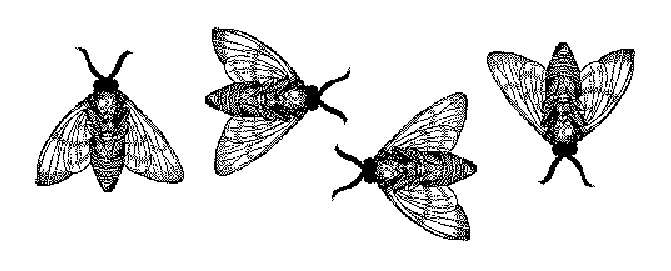
\epsfig{file=flies.eps}
\caption{A sample black and white graphic (.eps format)
that needs to span two columns of text.}
\end{figure*}

Note that either {\textbf{.ps}} or {\textbf{.eps}} formats are
used; use
the \texttt{{\char'134}epsfig} or \texttt{{\char'134}psfig}
commands as appropriate for the different file types.

%\begin{figure}
%\centering
%\psfig{file=rosette.ps, height=1in, width=1in,}
%%\caption{A sample black and white graphic (.ps format) that has
%been resized with the \texttt{psfig} command.}
%\vskip -6pt
%\end{figure}

\subsection{Theorem-like Constructs}
Other common constructs that may occur in your article are
the forms for logical constructs like theorems, axioms,
corollaries and proofs.  There are
two forms, one produced by the
command \texttt{{\char'134}newtheorem} and the
other by the command \texttt{{\char'134}newdef}; perhaps
the clearest and easiest way to distinguish them is
to compare the two in the output of this sample document:

This uses the \textbf{theorem} environment, created by
the\linebreak\texttt{{\char'134}newtheorem} command:
\newtheorem{theorem}{Theorem}
\begin{theorem}
Let $f$ be continuous on $[a,b]$.  If $G$ is
an antiderivative for $f$ on $[a,b]$, then
\begin{displaymath}\int^b_af(t)dt = G(b) - G(a).\end{displaymath}
\end{theorem}

The other uses the \textbf{definition} environment, created
by the \texttt{{\char'134}newdef} command:
\newdef{definition}{Definition}
\begin{definition}
If $z$ is irrational, then by $e^z$ we mean the
unique number which has
logarithm $z$: \begin{displaymath}{\log e^z = z}\end{displaymath}
\end{definition}

Two lists of constructs that use one of these
forms is given in the
\textit{Author's  Guidelines}.
 
There is one other similar construct environment, which is
already set up
for you; i.e. you must \textit{not} use
a \texttt{{\char'134}newdef} command to
create it: the \textbf{proof} environment.  Here
is a example of its use:
\begin{proof}
Suppose on the contrary there exists a real number $L$ such that
\begin{displaymath}
\lim_{x\rightarrow\infty} \frac{f(x)}{g(x)} = L.
\end{displaymath}
Then
\begin{displaymath}
l=\lim_{x\rightarrow c} f(x)
= \lim_{x\rightarrow c}
\left[ g{x} \cdot \frac{f(x)}{g(x)} \right ]
= \lim_{x\rightarrow c} g(x) \cdot \lim_{x\rightarrow c}
\frac{f(x)}{g(x)} = 0\cdot L = 0,
\end{displaymath}
which contradicts our assumption that $l\neq 0$.
\end{proof}

Complete rules about using these environments and using the
two different creation commands are in the
\textit{Author's Guide}; please consult it for more
detailed instructions.  If you need to use another construct,
not listed therein, which you want to have the same
formatting as the Theorem
or the Definition\cite{salas:calculus} shown above,
use the \texttt{{\char'134}newtheorem} or the
\texttt{{\char'134}newdef} command,
respectively, to create it.

\subsection*{A {\secit Caveat} for the \TeX\ Expert}
Because you have just been given permission to
use the \texttt{{\char'134}newdef} command to create a
new form, you might think you can
use \TeX's \texttt{{\char'134}def} to create a
new command: \textit{Please refrain from doing this!}
Remember that your \LaTeX\ source code is primarily intended
to create camera-ready copy, but may be converted
to other forms -- e.g. HTML. If you inadvertently omit
some or all of the \texttt{{\char'134}def}s recompilation will
be, to say the least, problematic.

\section{Conclusions}
This paragraph will end the body of this sample document.
Remember that you might still have Acknowledgments or
Appendices; brief samples of these
follow.  There is still the Bibliography to deal with; and
we will make a disclaimer about that here: with the exception
of the reference to the \LaTeX\ book, the citations in
this paper are to articles which have nothing to
do with the present subject and are used as
examples only.
%\end{document}  % This is where a 'short' article might terminate

%ACKNOWLEDGMENTS are optional
\section{Acknowledgments}
This section is optional; it is a location for you
to acknowledge grants, funding, editing assistance and
what have you.  In the present case, for example, the
authors would like to thank Gerald Murray of ACM for
his help in codifying this \textit{Author's Guide}
and the \textbf{.cls} and \textbf{.tex} files that it describes.

%
% The following two commands are all you need in the
% initial runs of your .tex file to
% produce the bibliography for the citations in your paper.
\bibliographystyle{abbrv}
\bibliography{sigproc}  % sigproc.bib is the name of the Bibliography in this case
% You must have a proper ".bib" file
%  and remember to run:
% latex bibtex latex latex
% to resolve all references
%
% ACM needs 'a single self-contained file'!
%
%APPENDICES are optional
%\balancecolumns
\appendix
%Appendix A
\section{Headings in Appendices}
The rules about hierarchical headings discussed above for
the body of the article are different in the appendices.
In the \textbf{appendix} environment, the command
\textbf{section} is used to
indicate the start of each Appendix, with alphabetic order
designation (i.e. the first is A, the second B, etc.) and
a title (if you include one).  So, if you need
hierarchical structure
\textit{within} an Appendix, start with \textbf{subsection} as the
highest level. Here is an outline of the body of this
document in Appendix-appropriate form:
\subsection{Introduction}
\subsection{The Body of the Paper}
\subsubsection{Type Changes and  Special Characters}
\subsubsection{Math Equations}
\paragraph{Inline (In-text) Equations}
\paragraph{Display Equations}
\subsubsection{Citations}
\subsubsection{Tables}
\subsubsection{Figures}
\subsubsection{Theorem-like Constructs}
\subsubsection*{A Caveat for the \TeX\ Expert}
\subsection{Conclusions}
\subsection{Acknowledgments}
\subsection{Additional Authors}
This section is inserted by \LaTeX; you do not insert it.
You just add the names and information in the
\texttt{{\char'134}additionalauthors} command at the start
of the document.
\subsection{References}
Generated by bibtex from your ~.bib file.  Run latex,
then bibtex, then latex twice (to resolve references)
to create the ~.bbl file.  Insert that ~.bbl file into
the .tex source file and comment out
the command \texttt{{\char'134}thebibliography}.
% This next section command marks the start of
% Appendix B, and does not continue the present hierarchy
\section{More Help for the Hardy}
The sig-alternate.cls file itself is chock-full of succinct
and helpful comments.  If you consider yourself a moderately
experienced to expert user of \LaTeX, you may find reading
it useful but please remember not to change it.
%\balancecolumns % GM June 2007
% That's all folks!

